\section{Theory}

In the automotive industry car companies are putting huge resources in optimising and developing new efficient processes that are in favour of the environment and the safety of the roads for autonomous cars. In this cluster of new technology there is a working concept called V2V \textit{(Vehicle-to-vehicle communication)}. V2V is a wireless transmission system that is used to give cars the possibility to communicate with each other for the purpose of reducing the risk of collision and also for more energy efficiency. The main data sent between the cars is speed, position and direction. This kind of information means that the V2V technology in theory can be modified to suit other road objects. Instead of communicating car to car only, this technology could be implemented between cars and the infrastructure as V2I or between cars and bikes as V2B. This gave the idea to the concept V2X \textit{("Vehicle-to-Everything")}. The goal of V2X is to reduce the total amount of car crashes in traffic by facilitating more data to the cars. This is especially valuable for the future as cars are becoming more and more autonomous. In the development of autonomous cars is where this project really enters the picture. In a world where cars are to communicate with each other, why not also have them communicate with everything else on the road.

\subsection{AD-HOC}
The data in V2V is sent over an AD-HOC network \textit{(See Figure 2}), which is a type of LAN \textit{(Local Area Network)} [2]. V2V is already implemented in the cars and used in the simulation environment OTTO so they already have a transmitter and a receiver. The figure shows how V2X could be used together with V2V in different potential products. A bike, traffic light and a construction site.

\begin{figure}[H]
    \centering
    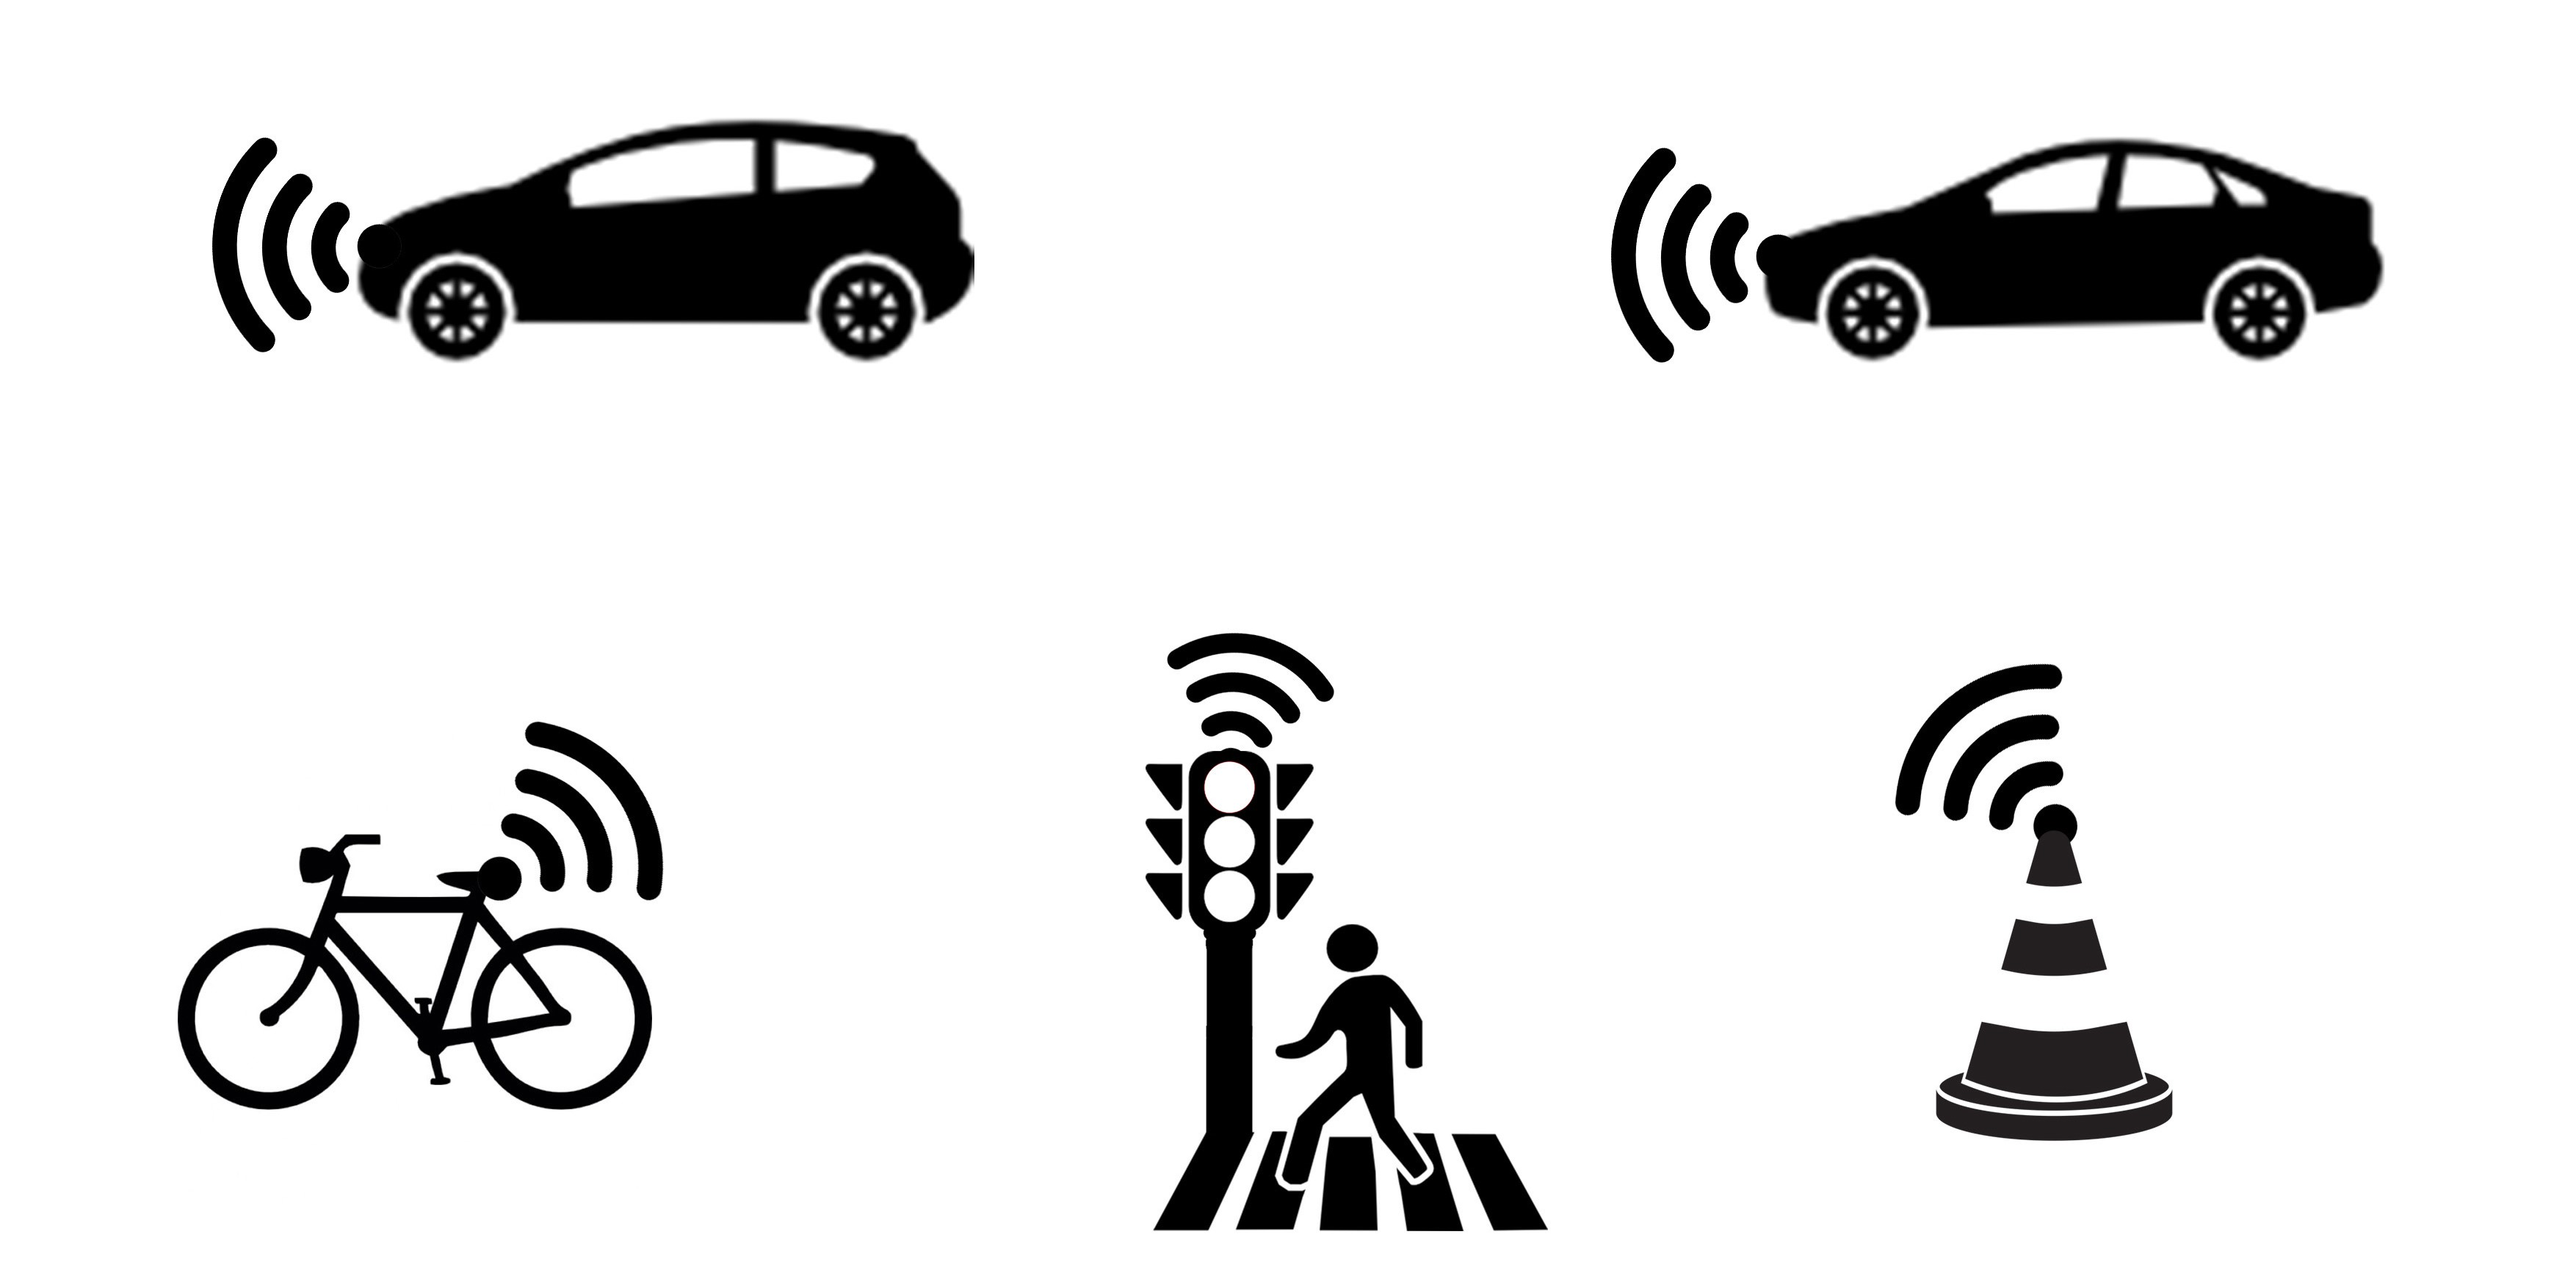
\includegraphics[scale=0.4]{images/projektsketch2.jpg}
    \caption{AD-HOC (LAN)}
\end{figure}

There is another potential type of service called WAN \textit{(Wide Area Network)} [3] that could be used, but the problem is that WAN has higher signal latency then LAN. Because the cars in traffic must react quickly, the higher latency in WAN could cause issues. It is also difficult to use in areas with bad connection to the grid. A global network would require that every car has to be connected via satellite \textit{(See Figure 3)} through some service or has a phone connected to the car. A method which is not reliable, because there would also need to be a big server-farm to coop with all the data. LAN is therefore a better choice since it is safer and the signal travel time is faster. 

\begin{figure}[H]
    \centering
    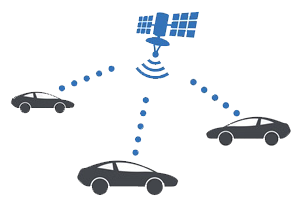
\includegraphics[scale=0.8]{images/V2VGlobal.png}
    \caption{Cloud network (WAN)}
\end{figure}

\subsection{ITS-G5}
The technology used is called "Cooperative Intelligent Transport Systems" C-ITS or ITS-G5 and is a broadcast technology based on the wireless standard 802.11p. It is the only validated and available technology in the market. It is capable of delivering secure AD-HOC direct with vehicle-to-vehicle and/or vehicle-to-infrastructure communication. The European Commission are creating a documentation on the ITS-G5 standard for EU \textit{"ITS-G5 is running in the designated 5.9 GHz frequency band that is foreseen for road safety"} [1]. This to set a standard on the framework for the future so that every manufacturer can build after the same regulations so that different cars and other road products with the V2X can cooperate with each other directly. 
